\documentclass[a4paper]{article}
\usepackage{amsmath}
\usepackage{amsfonts}
\usepackage{amsthm}
\usepackage{amssymb}
\usepackage[english]{babel}
\usepackage{float}
\usepackage{graphicx}
\usepackage{hyperref}
\usepackage[utf8]{inputenc}
\usepackage{listings}
\usepackage{xcolor}
%% \usepackage{subfigure}
\usepackage{graphicx}
\usepackage{subcaption}
\usepackage{stmaryrd}

\usepackage{a4wide}
\usepackage{url}

\usepackage{appendix}

\graphicspath{{imgs/}} %Setting the graphicspath

\lstset{
  frame=tb,
  language=Python,
  aboveskip=3mm,
  belowskip=3mm,
  showstringspaces=false,
  formfeed=newpage,
  tabsize=4,
  comment=[l]{\#},
  breaklines=true,
  morekeywords={models, lambda, forms}
}

\newcommand{\prob}[1]{\mathbb{P}\left(#1\right)}
\newcommand{\expect}[1]{\mathbb{E}\left(#1\right)}
\newcommand{\avg}[1]{\sum_{i=1}^{#1}X_i}
\newcommand*{\QEDA}{\hfill\ensuremath{\blacksquare}}%

\newcommand{\bt}{\textbf}
\newcommand{\nt}{\text}
\newcommand{\lagr}{\mathcal{L}}
\newcommand{\isum}{\sum^\infty_}
\newcommand{\f}{$f$}

\title{\vspace{-5cm} Numerical Optimization \\ Re-exam Handin 2}
\author{Dmitry Serykh (qwl888)}

\begin{document}
\maketitle
\section{The Setup}
For this assignment, I used Python, and all the relevant functions from
\texttt{numpy} and \texttt{scipy} packages. In particular, I have utilized the
\texttt{minimize} function from the \texttt{scipy.optimize} library.
I have chosen the BFGS optimizer, since
it is the default choice for the unconstrained optimization in this library. BFGS stands for
Broyden–Fletcher–Goldfarb–Shanno algorithm and belongs to the family
of quasi-Newton optimizers that is a state-of-the-art alternative to Newton
methods, thus it does not require the Hessian matrix. Moreover, it can be
classified as a Line-Search algorithm, where we first determine the direction
$p_k$ and the step length in that direction $\alpha$ afterwards.

\subsection{Parameters}
The \texttt{scipy} implementation of the BFGS algorithm has following
parameters:

\begin{itemize}
\item \emph{maxiter} - Maximum number of iterations to perform.
\item \emph{gtol} - Gradient norm must be less than gtol before successful termination.
\item \emph{norm} - Order of norm
\item \emph{eps} - Step size used when the gradient is approximated.
\end{itemize}
I used the value of $1000$ for the \emph{maxiter} parameter, but it was never
used, since the gradient magnitude was used as a primary stopping criterion.
For \emph{gtol}, I used the default value of
$10^{-5}$, and $\infty$ for the \emph{norm}. \emph{eps} was not used, since I we
have implemented a gradient for all five functions and we do not need to
approximate it. For all the functions, I have used a dimensionality of two.

\section{Testing}
\subsection{What constitutes a good testing protocol?}
According to Chapter 1 in the book, good optimization algorithms must have
following properties:
\begin{itemize}
\item \textbf{Robustness}. Ability of the algorithm to find minima of vast array
  of different functions. Furthermore, the algorithm should be indifferent to
  the starting point $x_0$.
\item \textbf{Efficiency}. A good optimization algorithm should not consume too
  much computational resources (and memory/storage).
\item \textbf{Accuracy}. Good optimization algorithms should find the minima
  accurately to some tolerance $\varepsilon$.
\end{itemize}
In order to process and then visualize the gathered data from the experiments, I
must use one of the existing aggregation methods. These include: minimum, maximum,
average(mean), median, variance, standard deviation. I decided both to use the
median and the mean. The main difference between these methods is how they
manage the influence of the outliers. When using the mean, we maintain the
influence of the outliers in the set, while it is excluded when using the median.

\subsection{My testing protocol}
In order to test the effectiveness of the BFGS implementation from the
\texttt{scipy.optimize}, I came up with a testing protocol:
\begin{itemize}
\item In order to measure the robustness of the algorithm, I have used the
  algorithm to find the minima of all five problem functions: The Ellipsoid
  function($f_1$), the Rosenbrock Banana function ($f_2$), The Log-Ellipsoid
  function ($f_3$) and the Attractive Sector functions ($f_4$ and $f_5$).
  To test if the algorithm is indifferent to the starting point $x_0$, I have
  used a random starting point taken from the uniform distribution in the
  interval between $-10$ to $10$ for both dimensions,
  repeated all the experiments 100 times and took the median of the results.
\item I decided to measure the efficiency of the algorithms in number of
  iterations until the gradient magnitude reaches $10^{-5}$. It should however
  be noted that steps of some algorithms are more
  computationally expensive than others. For example the Newton step requires a
  computation of Hessian and therefore more expensive than a steepest-descent step.
  The results can be seen on Table \ref{table}.
\item The accuracy of the algorithm was tested by measuring the Euclidean distance
  between the current point and the optima. The results can be seen on Table \ref{table}.
\item The convergence plots with the number of iteration on the x-scale and the
  Euclidean distance between the current value of $x$ and the
  optimum. The results can be seen on Figure \ref{plt1}.
\item The convergence plots with the gradient magnitude
  can be seen on Figure \ref{plt2}.
\end{itemize}

\begin{figure}[]
  \centering
  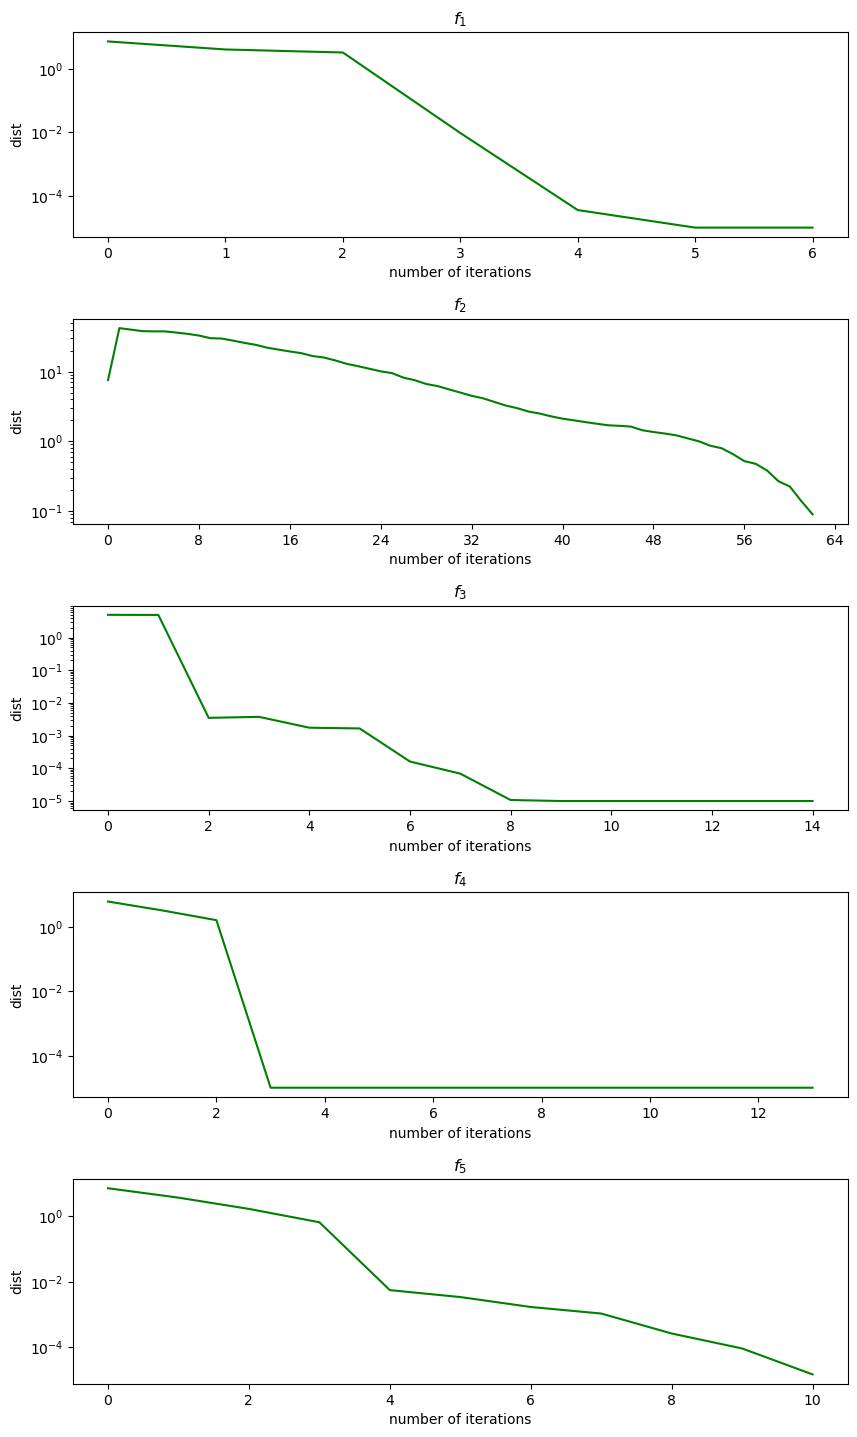
\includegraphics[width=0.8\textwidth]{plt_dists.png}
  \caption{Convergence Plot for BFGS, median of 100 runs. Y-axis shows the
    Euclidean distance to the optimum of each $f_1,...,f_7$ with random starting point}
  \label{plt1}
\end{figure}

\begin{figure}[]
  \centering
  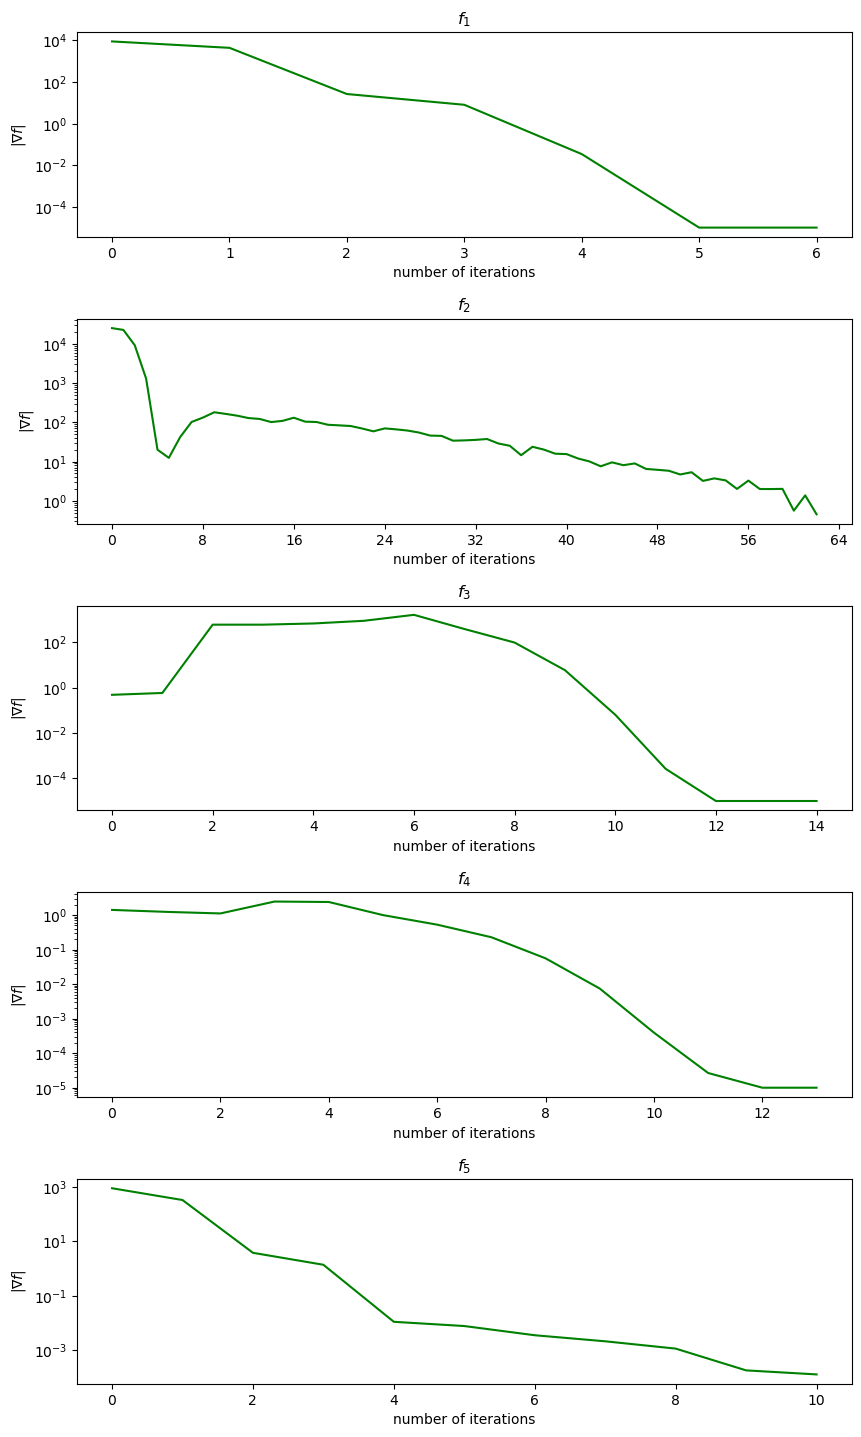
\includegraphics[width=0.8\textwidth]{plt_grad_norms.png}
  \caption{Convergence Plots for BFGS, median over 100 runs. Y-axis shows the
    norm of the gradient of each $f_1,...,f_7$ with random starting point}
  \label{plt2}
\end{figure}

\begin{table}[]
\centering
\begin{tabular}{|l|l|l|l|l|l|}
\hline
                 & $f_1$ & $f_2$   & $f_3$  & $f_4$  & $f_5$ \\ \hline
efficiency & $7$ & $68$ & $16$ & $14$ & $12$ \\ \hline
accuracy & $1.877e-8$  & $3.864e-7$ & $1.426e-13$  & $6.512e-7$  & $8.72e-5$ \\ \hline
\end{tabular}
\caption{Median number of iterations until algorithm termination ( $\| \nabla f \| < 1e-5$) and final distance to the optimum for 100 random starting points in the interval $[-10,10]$}
\label{table}
\end{table}

%% \begin{figure}[H]
%%   \centering
%%   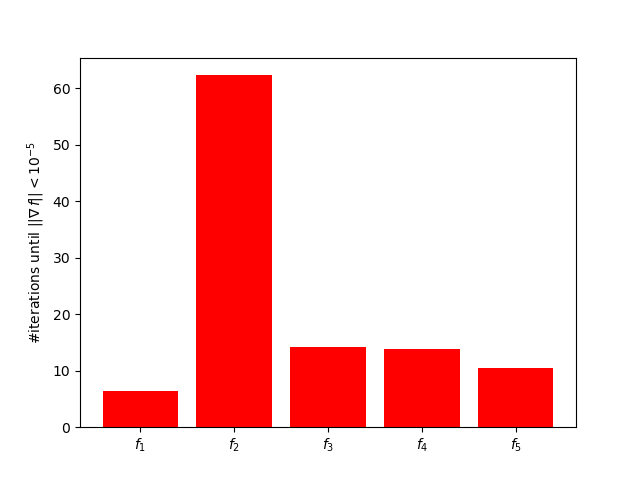
\includegraphics[width=\textwidth]{hist.png}
%%   \caption{Number of required iterations needed by BFGS to reach $||\nabla f|| < 10^{-5}$, averaged over 100 runs with random starting point}
%%   \label{plt2}
%% \end{figure}

\section{Theoretical Part}
\subsection{}
\subsubsection{}
Since $A \in \mathbb{R}^{d\times d}$ is invertible, $g(x) = Ax$ would constitute a linear map
$\mathbb{R}^n \rightarrow \mathbb{R}^n$. Linear transformations preserve the
ratios of lengths, therefore the inequality
\[
f(\alpha(A x)+(1-\alpha)(A y)) \leq \alpha f(A x)+(1-\alpha) f(A y), \text { for all } \alpha \in[0,1]
\]
would still hold, since we know that $f$ is strictly convex and therefore:
\[
f(\alpha(x)+(1-\alpha)(y)) \leq \alpha f(x)+(1-\alpha) f(y), \text { for all } \alpha \in[0,1]
\]
\subsubsection{}
We start by looking at an expression $x^TQx$. We know that $Q$ is symmetric
positive definite, hence we can use Cholesky decomposition and obtain following:
$x^TQx = x^TLL^Tx$, where $L$ is triangular matrix with positive diagonal
values, hence invertible.\\\\
Let $f(y) = y^Ty$, then $\nabla f(y) = 2y$ and $\nabla^2 f(y) = 2I$. $2I$ is
PD, therefore $f(y)$ is strictly convex. Then, if we set $y=L^Tx$,we get:
\[
f(y) = f(Lx) = x^TLL^Tx = x^TQx
\]
$x^TQx$ is therefore strictly convex, since $f(x)$ is convex and 
property from the previous subsection holds. \\\\
This point is relevant for quadratic-based functions such as $f_1$ and $f_2$,
where the convexity makes the optimizer converge on the optimum.

\subsection{}
\subsubsection{}
For $d=1$, the Log-Ellipsoid function could be formulated as:
\[
  f_3(x) = \log(\epsilon + x^2) 
\]
Hence, the derivatives:
\begin{align*}
  f_3'(x) &= \frac{2x}{\epsilon + x^2} \\
  f_3''(x) &= \frac{2(\epsilon - x^2)}{(\epsilon + x^2)^2}
\end{align*}
For $|x| < \epsilon$, $(\epsilon - x^2) > 0$, hence $f_3''(x) > 0$, and $f_3$
would be strictly convex.
\[
(-f_3)''(x) = \frac{2(x^2 - \epsilon)}{(\epsilon + x^2)^2}
\]
Hence, for $|x| \geq \epsilon$, $-f_3''(x) \geq 0$, which means that $-f_3$ is
convex, hence $f_3$ is concave for $|x| \geq \epsilon$.\\\\
This could potentially be problematic if the gradient-based optimizer gets its current value of
$x>|\epsilon|$, then it would fail finding an optimum, because it could continue
moving in that direction for an indefinite amount of time or until the number of
iterations reaches the predefined limit. 

\section{Conclusion}
Based on the results of application of the two performance metrics, the
\texttt{scipy} implementation of the BFGS optimizer managed to find the minima
of all case functions. It struggled most with the Rosenbrock function, due to its
elongated and curved iso-level.

\end{document}


%% \begin{figure}[h]
%%     \centering
%%     \subfloat[3d plot]{{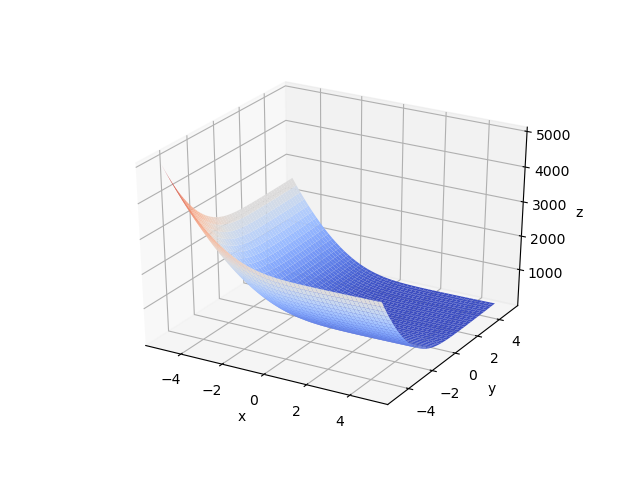
\includegraphics[width=6cm]{plt51.png} }}%
%%     \qquad
%%     \subfloat[Contour plot]{{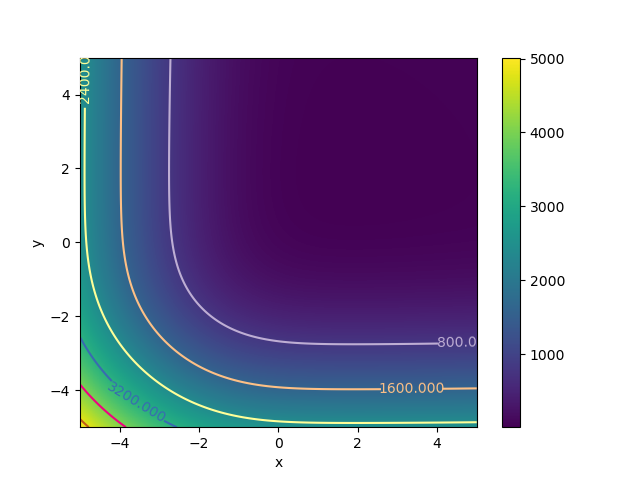
\includegraphics[width=6cm]{plt52.png} }}%
%%     \caption{The plots show the surface of the Attractive-Sector quadratic function}%
%%     \label{fig:5}%
%% \end{figure}

%% \section{Convergence Plots}
%% \label{sec:conv}
%% \begin{figure}[H]
%%   \centering
%%   \begin{subfigure}[b]{\textwidth}
%%     \centering
%%     \includegraphics[width=\textwidth]{plt_f_1.png}
%%     \caption{Ellipsoid Function}
%%   \end{subfigure}
%%   \begin{subfigure}[b]{\textwidth}
%%     \centering
%%     \includegraphics[width=\textwidth]{plt_f_2.png}
%%     \caption{Rosenbrock Function}
%%   \end{subfigure}
%%   \caption{Convergence Plots}
%%   \label{plt1}
%% \end{figure}
%% \end{document}
